\documentclass{article}

\usepackage[english]{babel}
\usepackage[utf8]{inputenc}
\usepackage{amsmath}
\usepackage{amsthm}
\usepackage{amssymb}
\usepackage{amsfonts}
\usepackage{bbm}
\usepackage{graphicx}
\usepackage{wrapfig}

% set up margin
\usepackage
[
  a4paper,
  left=3cm,
  right=3cm,
  top=3cm,
  bottom=3cm,
]
{geometry}

% set up header
\usepackage{fancyhdr}
\pagestyle{fancy}
\fancyhf{}
\lhead{6.438 Algorithms for Inference}
\chead{Problem Set 2}
\rhead{Hongzi Mao}
\cfoot{\thepage}

% footer line
\renewcommand{\footrulewidth}{0.4pt}

% sans serif italic
\newcommand{\s}[1]{\textsf{\textit{#1}}}

% set symbol
\usepackage[mathscr]{euscript}

% empty set
\let\emptyset\varnothing

% qed
\newcommand{\qeds}{\hfill\qedsymbol}

% independence symbol
\makeatletter
\newcommand*{\indep}{%
  \mathbin{%
    \mathpalette{\@indep}{}%
  }%
}
\newcommand*{\nindep}{%
  \mathbin{%                   % The final symbol is a binary math operator
    \mathpalette{\@indep}{\not}% \mathpalette helps for the adaptation
                               % of the symbol to the different math styles.
  }%
}
\newcommand*{\@indep}[2]{%
  \sbox0{$#1\perp\m@th$}%        box 0 contains \perp symbol
  \sbox2{$#1=$}%                 box 2 for the height of =
  \sbox4{$#1\vcenter{}$}%        box 4 for the height of the math axis
  \rlap{\copy0}%                 first \perp
  \dimen@=\dimexpr\ht2-\ht4-.2pt\relax
  \kern\dimen@
  {#2}
  \kern\dimen@
  \copy0 %                       second \perp
} 
\makeatother

%%%%%%%%%%%%%%%%%%%%%%%%%%%%%%%%%%%%%%%%%%%%%%%%%%%%%%%%%%%%%%%%%%%%%%%%
%%%%%%%%%%%%%%%%%%%%%%%%% Begin document here %%%%%%%%%%%%%%%%%%%%%%%%%%
%%%%%%%%%%%%%%%%%%%%%%%%%%%%%%%%%%%%%%%%%%%%%%%%%%%%%%%%%%%%%%%%%%%%%%%%
\begin{document}
 
\section*{Problem 2.2}
%
(a) To prove the largest clique size in $\mathscr{H}$ is $\max_i |\mathscr{S}_i| +1$,
we show 
\begin{enumerate}
	\item at every elimination step $i$, the newly generated edges and the eliminated edges to node $i$ forms a clique in $\mathscr{H}$;
	\item such clique has size $|\mathscr{S}_i| +1$; and
	\item the largest clique formed at the eliminated steps is no smaller than the largest clique in the reconstituted graph $\mathscr{H}$.
\end{enumerate}
%
\begin{figure}[h]
  \centering
  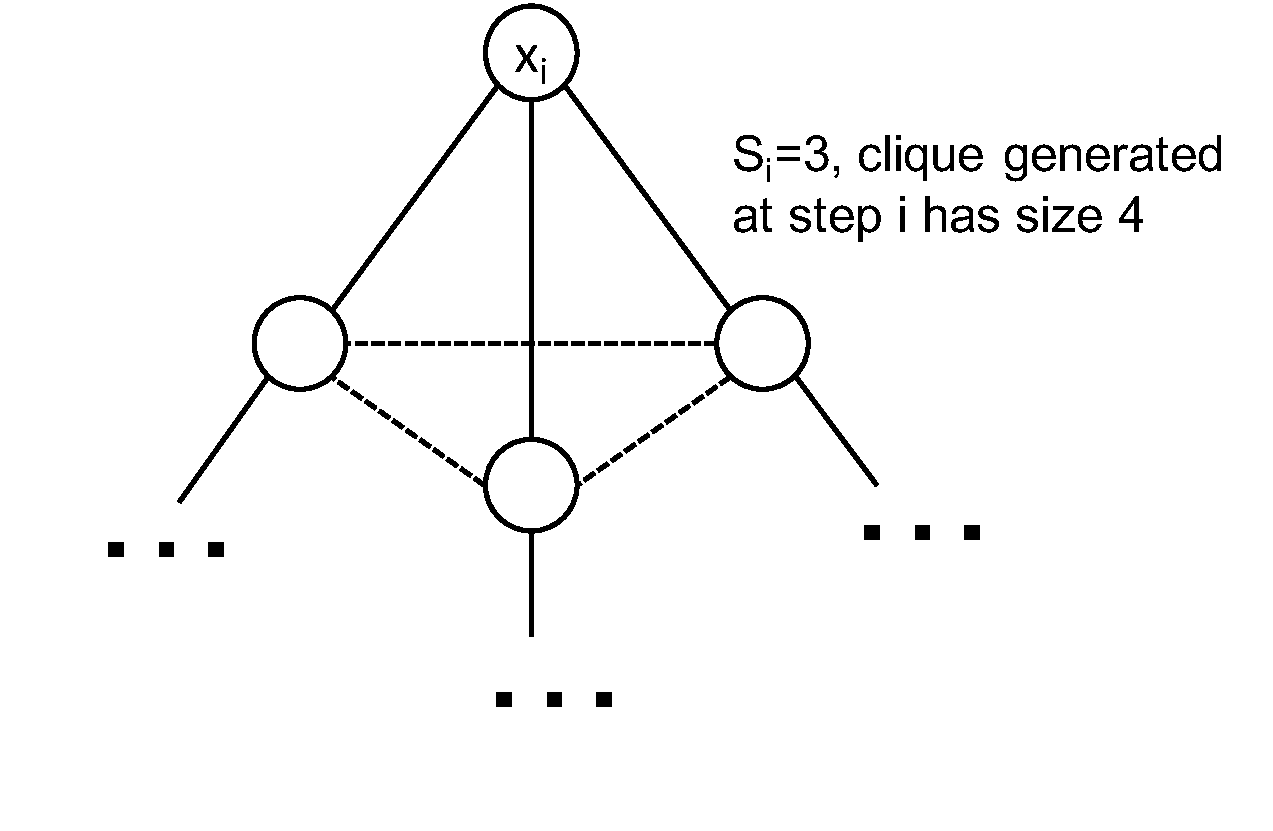
\includegraphics[width=0.5\columnwidth]{2a.pdf}
  \vspace{-0.7cm}
  \caption{Eliminating node $i$.}
  \label{f:2a}
\end{figure}
%

To show (1), we note that nodes in $\mathscr{S}_i$ are fully connected (dashed line in Figure~\ref{f:2a}) at elimination step $i$ (direct consequence of elimination). Since node $i$ was connected to all nodes in $\mathscr{S}_i$ (solid line connected to $i$ in Figure~\ref{f:2a}), this nodes set forms a clique.
%
For (2), the size of such clique at each step $i$ is all the uneliminated nodes connected to $i$ and node $i$ itself, i.e., $|\mathscr{S}_i| +1$.

%
To show (3), we first notice that the largest clique formed at elimination steps is no smaller than the largest clique in the \emph{original} graph $\mathscr{G}$. This is because, at the first time we eliminate any node $j$ in the largest clique of $\mathscr{G}$, the size $|\mathscr{S}_j|$ is at least the clique size $-1$ (as $j$ can only be connected with more nodes than all the nodes in the clique).

%
Second, the cliques with newly generated edges in $\mathscr{G}$ are formed in single elimination steps. This can be proved by contradiction. Suppose a clique in $\mathscr{G}$ is formed in multiple elimination steps. In such a clique, there exists a node \emph{not} connecting to all other nodes in the clique at its elimination step (otherwise a single step would have formed the clique). But after eliminating this node, other nodes have no way to form a connection with it, and thus can not form a clique with this node, which is a contradiction. Thus the largest clique in $\mathscr{H}$ is generated in a \emph{single} elimination step.

Therefore, the largest clique generated at the elimination steps, i.e., with size $\max_i |\mathscr{S}_i| +1$, is the largest clique in $\mathscr{H}$. \qeds
\\

%
\noindent
(b) We show $\mathscr{H}$ is chordal by induction.
%
For any cycle in $\mathscr{H}$ of size $4$, when eliminating any of the node will add in an edge (if not already exist) between its adjacent nodes, which makes makes this cycle chordal in $\mathscr{H}$.

%
Assume any cycle in $\mathscr{H}$ with size $N$ or less is chordal. For a cycle in $\mathscr{H}$ with size $N+1$, if there are existing edges connecting any nodes in the cycle, the cycle can be decomposed into multiple cycles with size strictly less than $N+1$. For all these cycles, they are chordal since their sizes are $N$ or less. If there is no previous edge in the cycle, eliminating any node will connect its adjacent nodes, making a triangle and a cycle with size $N$. Since the cycle with size $N$ in $\mathscr{H}$ is chordal and the triangle connects the 2 non-consecutive edges are connected in the triangle, the cycle with size $N+1$ is chordal. 

%
Therefore, by induction, $\mathscr{H}$ is chordal. \qeds

\pagebreak

%%%%%%%%%%%%%%%%%%%%%%%%%%%%%%%%%%%%%%%%%%%%%%%%%%%%%%%%%%%%%%%%%%%%%%%%%%%%%%%%%%%%%%%%
\section*{Problem 2.3}


\end{document}